\section{\textsf{REAR:} a framework for virtual exocentric vision systems}
\label{sec:rear}
In this section we will describe \textsf{R.E.A.R.} - 
\textit{Rear Exocentric Augmented Reality}, a framework 
for the development of virtual exocentric vision systems.
%
It has been written in C++, following an object-oriented 
approach, and implements the minimal set of tools and functionalities 
needed to create representations of a mobile robot in its environment 
through the use of augmented reality techniques, as described in 
section \ref{sec:exo}.
%

%
For what concerns graphics, \textsf{R.E.A.R.} relies on OpenGL.
It makes use of three software components: a \textit{camera}, 
a 3D model of the \textit{robot} itself and a \textit{texture}.
%
The camera provides the user with a view of the OpenGL space 
from a certain point-of-view and with a certain field-of-view. 
It identifies a \textit{viewing frustum} - as shown in figure 
\ref{fig:openglspace} - whose volume corresponds to the 
portion of OpenGL space displayed on the user's screen.
%
To give the user the illusion of seeing the robot from an 
external point-of-view, the 3d model of the robot is drawn 
within the viewing frustum, while the more distant frustum base 
is applied a texture displaying a picture previously 
captured from the robot's egocentric camera.
%

%
An example of what a user sees is showed in figure \ref{fig:snap}.
%
\begin{figure}[!h]
  \begin{center}
    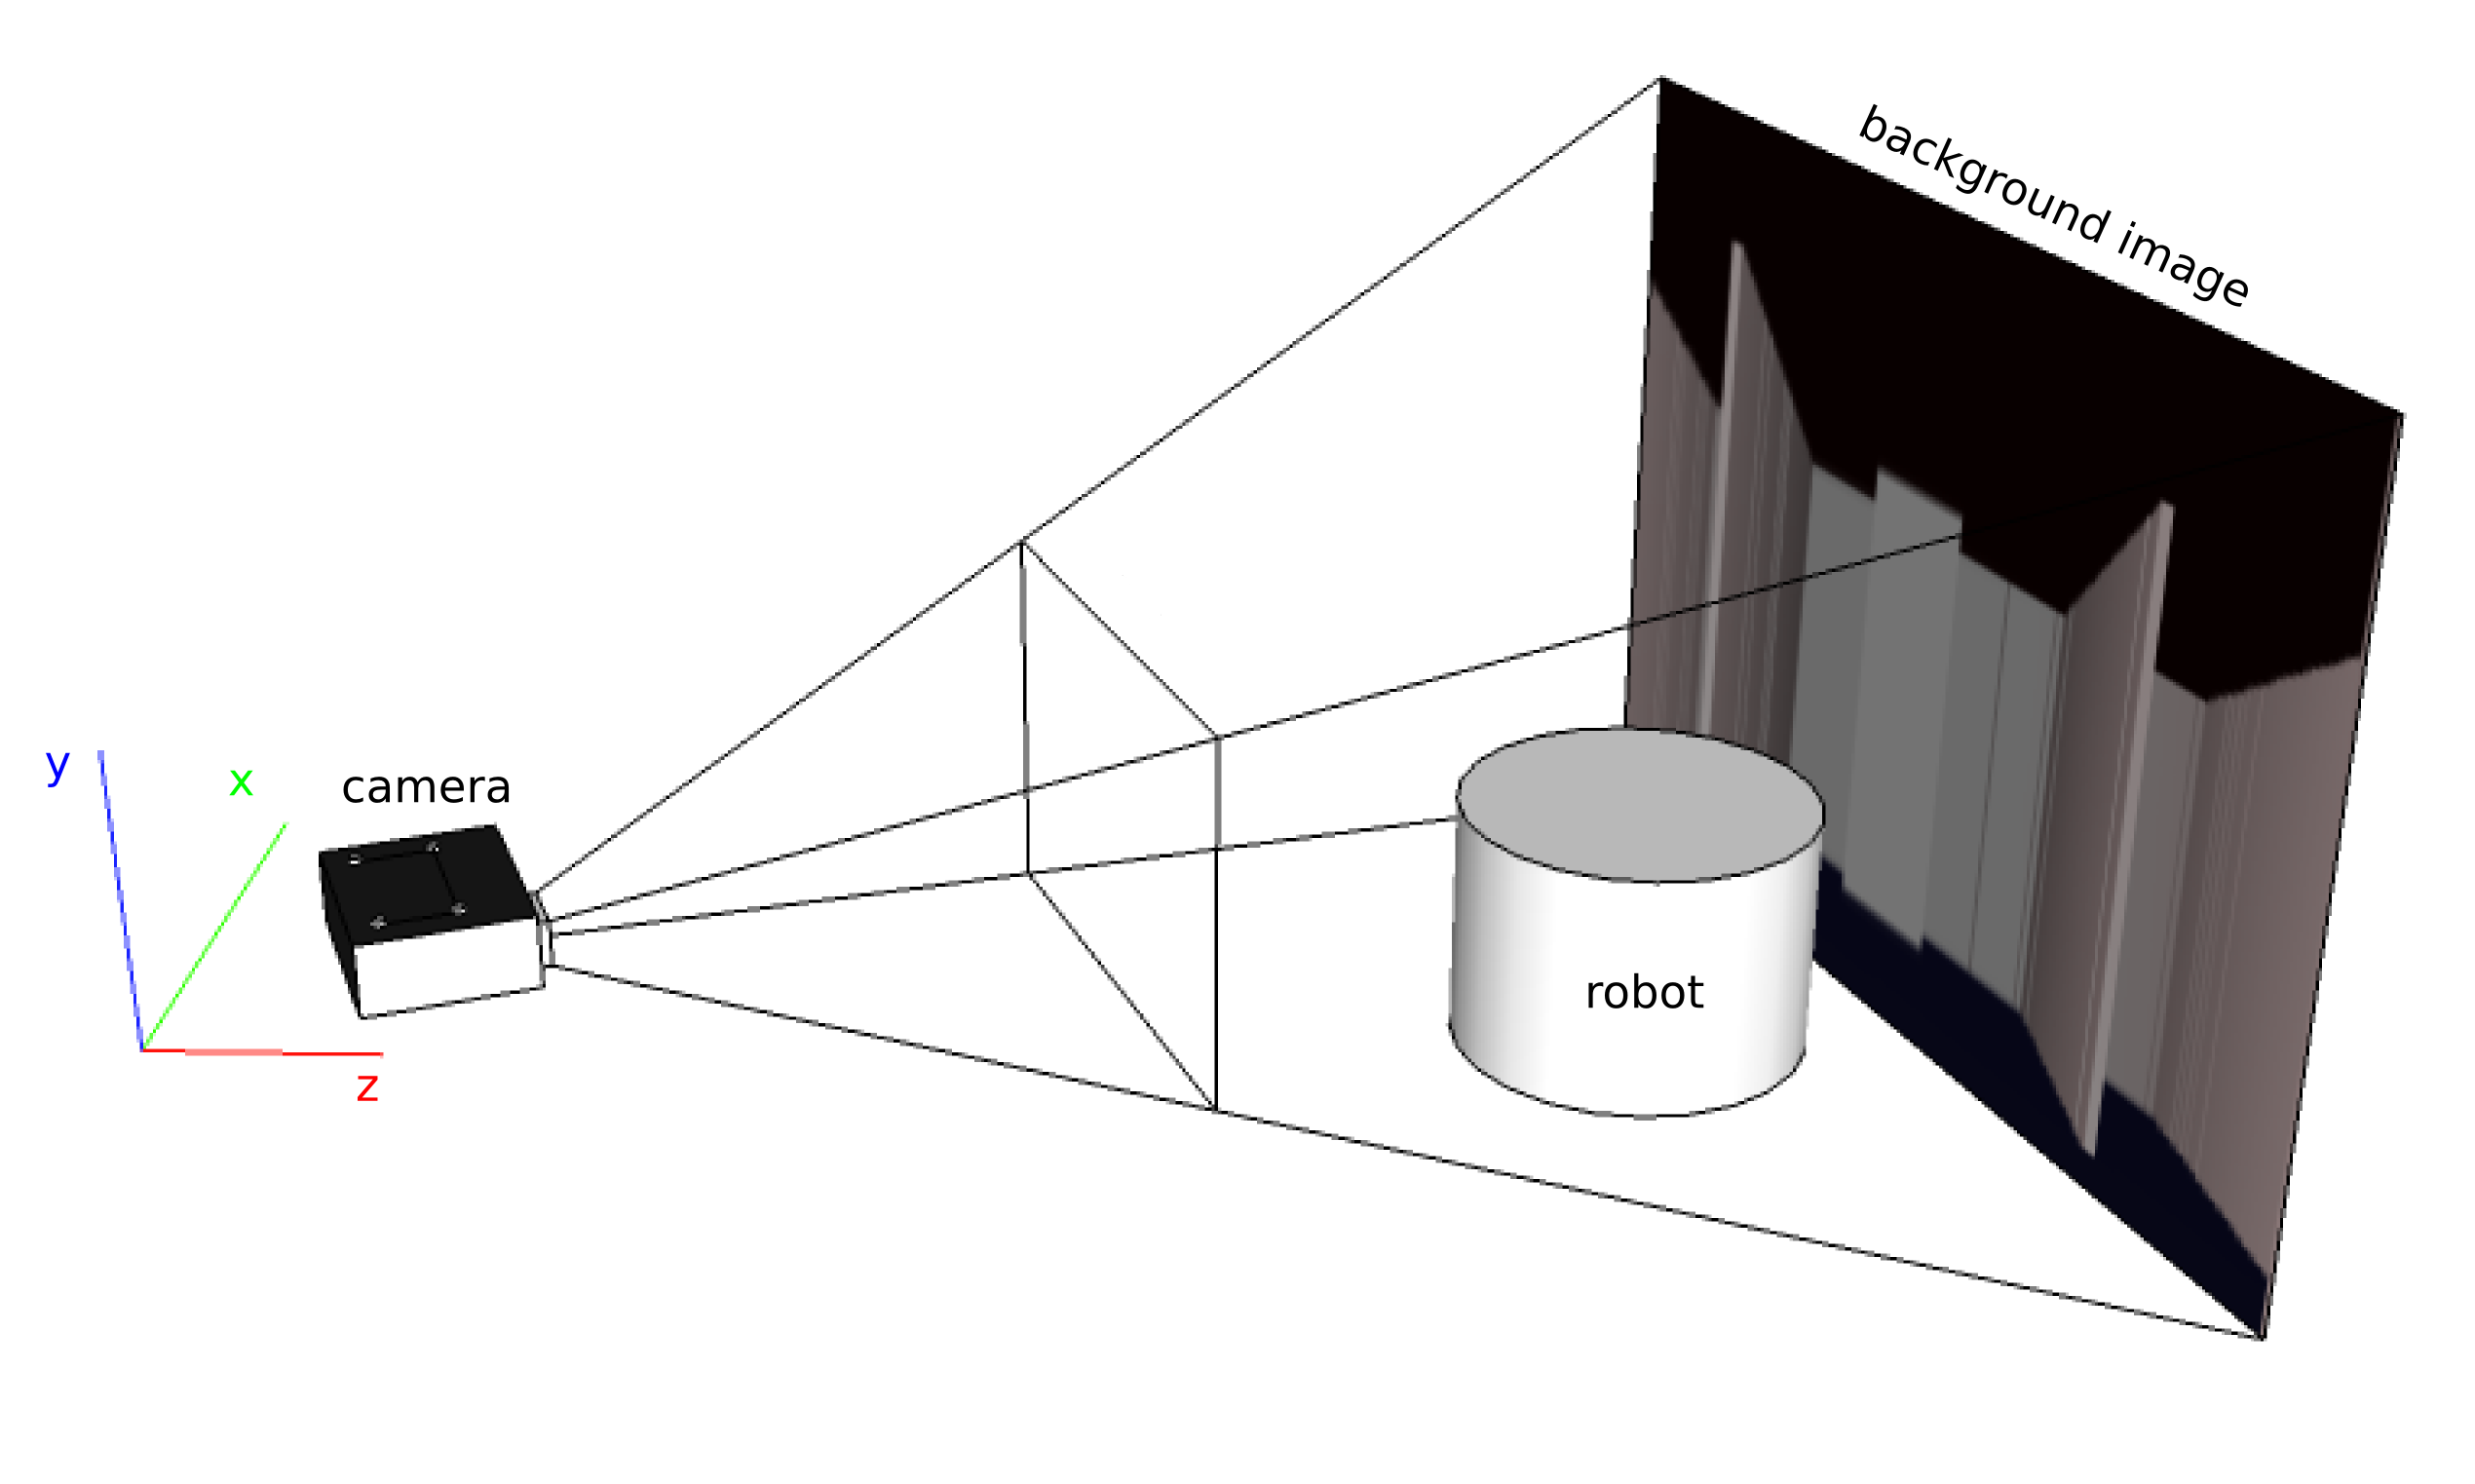
\includegraphics[width=300pt]{img/camera_frustum_scheme.png}
    \caption{The OpenGL space}
    \label{fig:openglspace}
  \end{center}
\end{figure}
%
\begin{figure}[!h]
  \begin{center}
    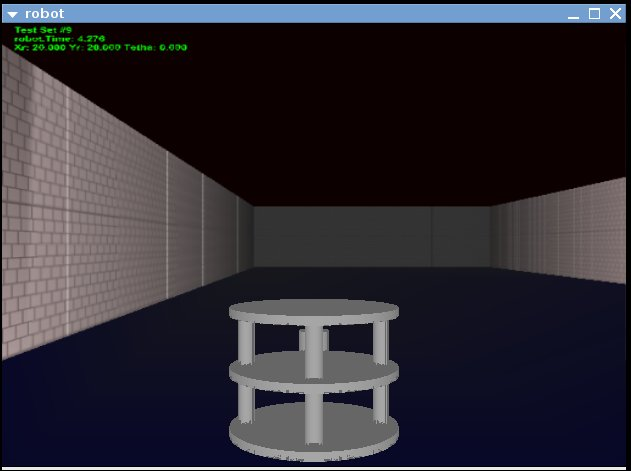
\includegraphics[width=300pt]{img/rear_snapshot_large.jpg}
    \caption{A snapshot from a \textsf{R.E.A.R.}-based application}
    \label{fig:snap}
  \end{center}
\end{figure}
%

%
Main issues in the approch we have just described are 1. 
\textit{where} to draw the robot within the viewing frustum 
and 2. \textit{which} of the captured images is to be used 
as background.
%
For what concerns the first issue, one can intuitively guess 
that the simplest way to determine the robot position 
within the frustum is to know the current robot position 
and orientation and the position and orientation of the egocentric 
camera when the snapshot was taken and, then, to set the 
position of the 3d model of the robot and the point-of-view 
of the camera accordingly.
Well, that's what \textsf{R.E.A.R.} does.
%
Therefore, to run, every \textsf{R.E.A.R.} concrete implementation 
needs, at least:
%
\begin{itemize}
  \item a set of snapshots captured from the robot egocentric camera, 
    together with the robot position at the time it was taken
  \item the robot's current position
\end{itemize}
%
Such data is retrieved every time the operator, using the 
interface provided by \textsf{R.E.A.R.} itself, sends a 
motion command to the robot.
%
Only once new data is collected, \textsf{R.E.A.R.} chooses 
an image to set as background and draw the robot model within 
the frustum. So, for what concerns issue no. 2, as already 
underlined in \cite{sugimoto}, let us say that there is not 
a \textit{unique} way to determine which image is to be set 
as background, since different image selection algorithms 
would differently affect user perceptions and. We will have a 
deeper look at some image selection algorithms in section
\ref{sub:howbackgroundimage}.
%
Finally, the overall execution loop is resumed by the flowchart 
showed in figure \ref{fig:overall_diagram}.
%
\begin{figure}[!h]
  \begin{center}
    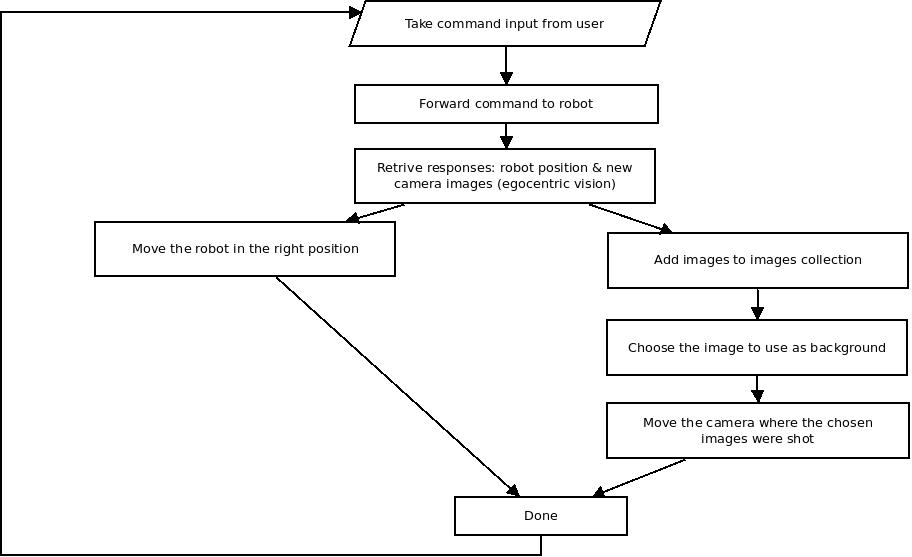
\includegraphics[width=350pt]{img/overall_diagram.jpeg}  %robot pic
    \caption{Application flowchart}
    \label{fig:overall_diagram}
  \end{center}
\end{figure}
%
%% The overall schema can be resumed by the following diagram (see figure
%% \ref{fig:overall_diagram}). User sends a command to the exocentric vision
%% application, in order to guide the robot through the remote environment.
%% The exocentric vision application forwards the command to the robot or the
%% simulator (paragraph \ref{sec:simulator}) and waits for the response.
%% The latter includes the new robot position and the new egocentric camera images.
%

%
%% All the egocentric camera images retrieved are stored in a data set and coupled
%% with robot coordinates and orientation at the moment when they were shot. Going
%% on with the application a large collection of egocentric images will be gathered.
%% %
%% Since every image owns its data about position and orientation when shot, we can
%% move and point the camera object to obtain the right visual of the external world.
%% Wherever the robot is situated, we will be able to watch it from the right point of view,
%% depending on the texture image chosen.
%% %

%% %
%% All the process explained above is lacking of one part: how to choose the background image,
%% knowing the actual robot position and orientation. If we decided to choose the closest image
%% to the robot we would always show the egocentric vision, because the algorithm would select
%% always the image with the same position and orientation of the robot. The distance between
%% the robot and the selected images would be equal to zero, which is doubtless the minimum possible
%% value.
%% %

%% %
%% The algorithms to take the right image in exocentric vision can be various. Each one has its own
%% advantages and disadvantages, we will chose the one able to guarantee the best trade-off.
%
%
\subsection{Class diagram}
%
Let us have a look at \textsf{R.E.A.R.} class diagram, 
showed in figure \ref {fig:class_diagram}.
%
\begin{figure}[!h]
  \begin{center}
    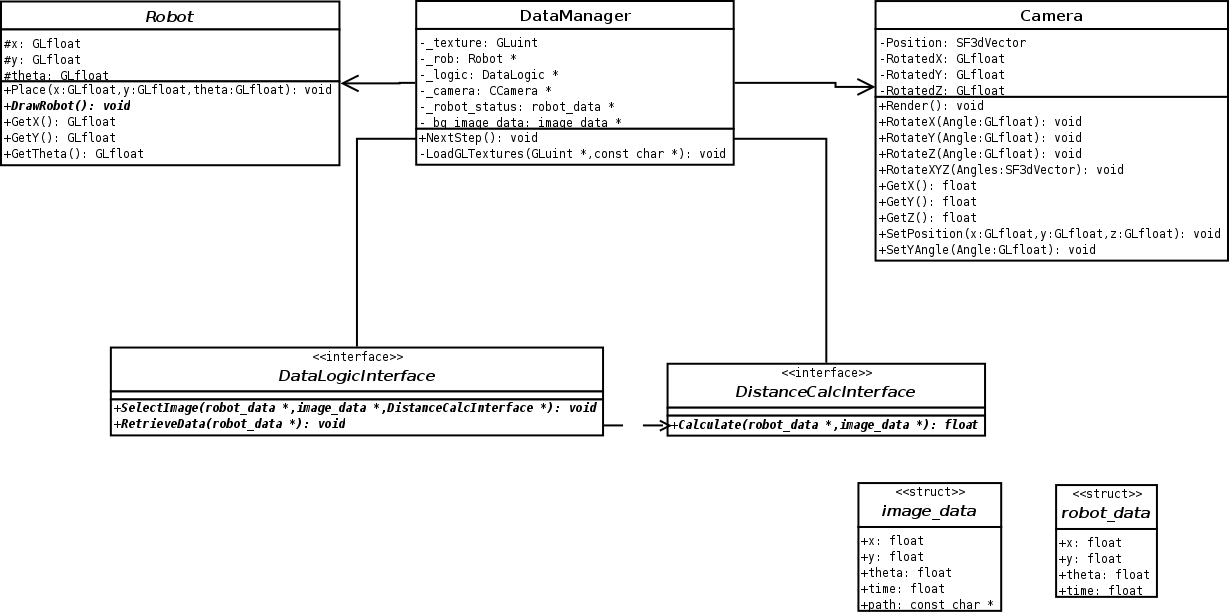
\includegraphics[width=400pt]{img/rear_class_diagram.png}
    \caption{\textsf{R.E.A.R.} class diagram}
    \label{fig:class_diagram}
  \end{center}
\end{figure}
%
Two of the components needed by \textsf{R.E.A.R.}, the robot 
model and the camera, are mapped on two dedicated classes, 
\texttt{Robot} and \texttt{Camera}, respectively.
%

%
The former is an \textit{abstract class}, serves as a storage 
for the current position and orientation of the actual
robot and declare a pure virtual method in which subclasses 
must include all of the procedure to draw the OpenGL model 
of the robot itself.
%
The latter is instead a \textit{helper class}, since there 
exists no actual camera within the OpenGL space. The camera 
model is just an abstraction used to give a more intuitive
way to set the portion of space the user is looking at.
In fact, the \texttt{Camera} class provides methods to 
set the user's point-of-view within the OpenGL space.
%

%
In the middle, between \texttt{Robot} and \texttt{Camera},
there is the \texttt{DataManager} class. It is intended to be 
the core of every \textsf{R.E.A.R.} based application, since it 
internally implements the loop showed in figure 
\ref{fig:overall_diagram}.
It acts as a \textit{mediator} among all of the other classes, 
in that it manages their interaction and, hence, reduces 
coupling between them.
%

%
The diagram also features two interfaces that have to be implemented 
by programmers who want to create their own concrete exocentric 
vision system: \texttt{DataLogicInterface} and 
\texttt{DistanceCalcInterface}.
%

%
The former decouples the application 
core, that is the \texttt{DataManager}, from the data source.
This way, \texttt{DataManager} code can be totally unaware of 
the technology used to retrieve data from the robot - e.g. 
sockets, web services, etc.
%

%
\texttt{DistanceCalcInterface}, instead, defines the interface 
of the component which implements the image selection algorithm.
%
In this case, the use of an interface leaves programmers 
able to change, and even to implement new image 
selection algorithms without having to worry about
changing other classes.
%

%
Finally, the class diagram presents two structures, 
\texttt{image\_data} and \texttt{robot\_data}, whose 
declarations are reported in listing \ref{code:data}.
%
The former is used to store all the metadata 
relative to a specific snapshot - i.e. the position 
and the orientation of the camera when it was taken, 
a timestamp and an array of chars that can be used by 
programmers who would like to add other data - e.g. 
a code or a sequence number.
%

%
The latter is similar to the former, it is meant to be 
used by \texttt{DataManager} to exchange informations
about the current robot position and orientation with 
lower-level objects, in a compact way.
%
\begin{lstlisting}[caption={\textsf{R.E.A.R.} data structures}, label={code:data}, frame=trBL]
struct image_data {
  float x;
  float y;
  float theta;
  float time;
  char path[100];
};

struct robot_data {
  float x;
  float y;
  float theta;
  float time;
};
\end{lstlisting}
%

%
In the following of this section, we will have a look 
\textit{under the hood} of the classes and interfaces 
we have just introduced.
%
We will see how \textsf{R.E.A.R.} functionalities are 
mapped onto them and, then, how to correctly subclass/use
them in order to build a concrete exocentric vision system.
%

%
\subsubsection{The Robot Class}
\label{sub:robotclass}
Let us have a look at the declaration of the \texttt{Robot}
class, reported in listing \ref{code:robot_class}.
%
\begin{lstlisting}[caption={\texttt{Robot} class declaration}, label={code:robot_class}, frame=trBL]
class Robot
{
 private:
  GLfloat x;
  GLfloat y;					
  GLfloat theta;

 public:
  Robot();
  GLfloat GetX();
  GLfloat GetY();
  GLfloat GetTheta();
  void Place(GLfloat x, GLfloat y, GLfloat theta);
  virtual void DrawRobot() = 0;
};
\end{lstlisting}
%
As already stated, private attributes of \texttt{Robot} 
are used to store the current position and orientation 
of the actual robot. Such attributes are initialized with 
all-zeros by the constructor, can be read by means 
of invoking their \textit{getter} methods and can be set 
by means of the \texttt{Place()} method.
%

%
\texttt{Robot} also declares an abstract \textit{hook} method, 
\texttt{DrawRobot()}. Such a method is called by the 
\texttt{DataManager} every time it wants to render the 
robot model and, hence, programmers who wants to 
use \textsf{R.E.A.R.} for their own robot should subclass 
\texttt{Robot} and implement \texttt{DrawRobot()} as a 
procedure that draws their custom robot model using 
the OpenGL API.
%
When doing that, one must always keep in mind that 
\textsf{R.E.A.R.} makes use of a three-dimensional OpenGL 
space, while position information is often represented 
as a \texttt{(x,y)} pair. \texttt{R.E.A.R.} maps the \texttt{x} 
value of such a pair onto the x axis of its OpenGL space, 
while the \texttt{y} value is mapped onto the z axis.
%
That is, the actual XY plan corresponds to the OpenGL 
XZ plan. Such a correspondence is represented in figure 
\ref{fig:reference_systems}.
%
\begin{figure}[!h]
  \begin{center}
    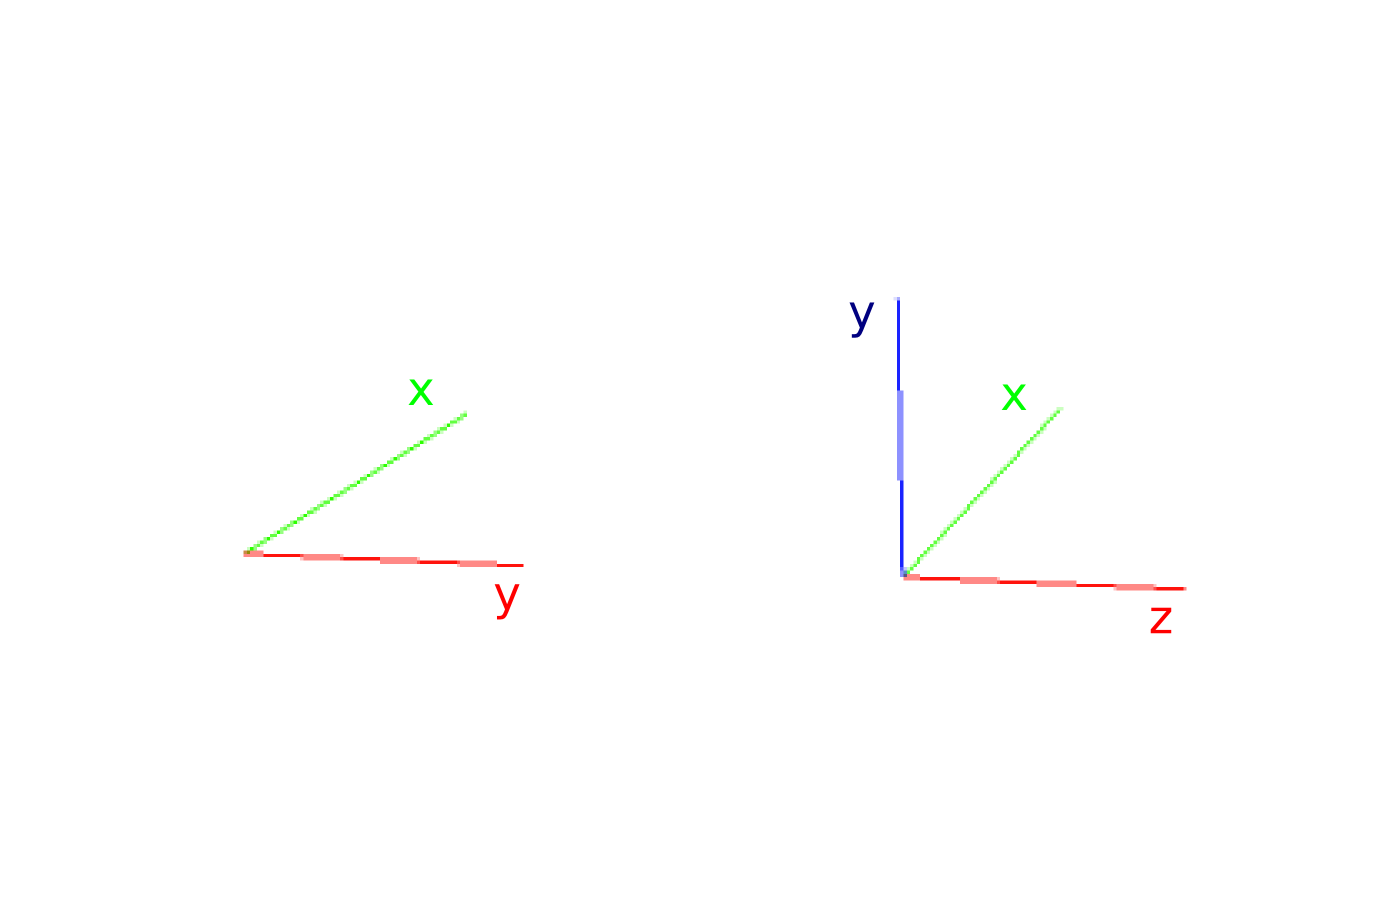
\includegraphics[width=300pt]{img/reference_system.png}
    \caption{Reference systems}
    \label{fig:reference_systems}
  \end{center}
\end{figure}
%

%
Moreover, to draw the robot in the right position within 
the OpenGL space, the first thing a \texttt{DrawRobot()} should 
do is to invoke OpenGL function \texttt{glTranslate()}.
%

%
A skeleton of a concrete implementation of \texttt{DrawRobot()}
would look like this:
\begin{lstlisting}[caption={\texttt{Robot} class declaration}, label={code:robot_class}, frame=trBL]  
  glMatrixMode(GL_MODELVIEW);
  glPushMatrix();

  // set robot position
  glTranslatef(this -> x, 0.0f, this -> y);

  // rotate the robot 
  glRotatef(this -> theta, 0.0f, 1.0f, 0.0f);

  // code to actually draw the robot

  glPopMatrix();
\end{lstlisting}
%

%
%  take the robot one step higher if it fails to be seen
% 
%% Both classes represent the 3morduc robot in openGL world. 
%% This means that the robot class offers, among others, a
%% method with the purpose of drawing itself, called by the 
%% OpenGL framework when it is necessary. The operation of 
%% drawing is completed thanks to other two methods, able 
%% to draw the elementary part of the robot - e.g. cylinders and disks.
%

%
%% There are not considerable different between the tho 
%% drawing method implantation. The main one is that in the 
%% new method, before starting drawing, the model-view matrix 
%% is copied in order to restore it at the end of the process. 
%% In these way we do not affect the model-view matrix status 
%% by drawing the robot.
%% %

%% %
%% The robot class, after the refactoring process, loses many 
%% of its public attributes and methods, so in the
%% exocentric vision control it is much more simple than the 
%% original one. First of all, the new class does not contain either
%% attributes to store the actual speed vector component, or 
%% a chronometer object to count the time, or information about wheels
%% encoder. This information was stored in the simulator robot 
%% class to calculate the position of the robot after a movement,
%% but since we retrieve the position directly from the simulator 
%% these fields are now useless. 
%

%
%% The unique attribute (changed from public to private, in 
%% the new version) which survives the refactory - along with the
%% triple values indicating coordinate on x axis, coordinate on 
%% y axis and rotation - is named \texttt{radius}. \texttt{radius}
%% is a float attribute, which stores the value of the radius for the 
%% tree cylinders which make up the robot. See figure
%% \ref{fig:3morduc_opengl} for a better understanding.
%% %
%% \begin{figure}[!h]
%%   \begin{center}
%%     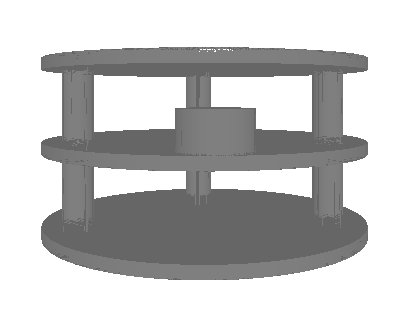
\includegraphics[width=200pt]{img/3morduc_opengl.png}  %robot pic
%%     \caption{The 3morduc robotic platform drawn in OpenGL}
%%     \label{fig:3morduc_opengl}
%%   \end{center}
%% \end{figure}
%% %
%% The default \texttt{radius} value is 4, but it can be 
%% customised by the user: by increasing it the robot will be 
%% displayed larger and larger on the screen, and viceversa.
%% %

%% %
%% All the attributes are private in the new robot class, 
%% so a method to get each one value is declared. 
%% %

%% %
%% Most of the previous public methods have been removed too. 
%% The constructor method, for instance, is present with one
%% only definition and default parameters, instead of declaring 
%% it twice (with parameter and without). The methods to set
%% linear and angular velocity are not present anymore, for 
%% the reason explained above; those to increment the collisions 
%% number are actually disabled because, at this development 
%% stage, the exocentric vision control does not face the collision 
%% problem. Anyway, it is supposed to cope with collision in 
%% the future version.
%% %

%% %
%% Besides, the method used by Privitera's simulator to read 
%% the robot initial position from file has been removed, since 
%% for the exocentric vision system robot always starts from 
%% fixed coordinates and rotation.
%% %

%% %
%% Finally, the method named with the signature 
%% \texttt{void move()} has been changed in \texttt{void Place(float x, float y, float theta)}
%% in order to set the x and y coordinate and the rotation of the robot. 
%% We remind that in the previous version these attributes
%% were public, so there were no need to pass them as parameters function.
%

%
\subsubsection{The Camera Class}
\label{sub:cameraclass}
OpenGL does not provide any \textit{camera}, anyway it proved 
to be extremely useful to have a helper class that permits 
to easily set position and orienation of the user's 
point of view and sight, without worrying about lower-level 
OpenGL details.
%

%
A basic implementation of such a helper class is suggested 
in \cite{opengl:camera}. Such an implementation is slightly 
similar the one featured by \textsf{R.E.A.R.}, whose 
declaration is reported in listing \ref{code:camera_class}.
%
\begin{lstlisting}[caption={\texttt{Camera} class declaration}, label={code:camera_class}, frame=trBL]
class Camera
{
 private:
  SF3dVector Position;
  GLfloat RotatedX, RotatedY, RotatedZ;	
  GLfloat _theta;

 public:
  Camera();
  void Render ( void );
  void Move ( SF3dVector Direction );
  GLfloat GetX();
  GLfloat GetY();
  GLfloat GetZ();
  GLfloat GetTheta();
  void SetPosition(GLfloat x, GLfloat y, GLfloat z);
  void SetYAngle ( GLfloat Angle );
  void RotateX ( GLfloat Angle );
  void RotateY ( GLfloat Angle );
  void RotateZ ( GLfloat Angle );
  void RotateXYZ ( SF3dVector Angles );
};
\end{lstlisting}
%
The \texttt{Camera} class allows to move and rotate the user 
point of view, independently from the robot.
%
This is essential for our purposes, since \textsf{R.E.A.R.}
must be able to draw the robot everywhere in the OpenGL space, 
regardless of where the camera is, and vice versa.
%

%
\texttt{Camera} methods are pretty simple: they just make 
use of OpenGL basic commands (such as \texttt{glTranslate} 
and \texttt{glRotate}) to actually move the OpenGL reference 
system and, hence, move the point-of-view and change the sight 
direction.
%
The only thing to care about when using such a class is 
to invoke the OpenGL commands \texttt{glMatrixMode(GL\_MODELVIEW)} 
and \texttt{glLoadIdentity()} before invoking its 
\texttt{Render()} method. This avoids previous modifications 
of the \texttt{GL\_MODELVIEW} matrix from affecting the 
positioning of the camera.
%

%
\subsubsection{The DataManager Class}
\label{sub:datamanager}
As already stated, the \texttt{DataManger} class is the \textit{core}
of the whole framework. Its declaration is reported in 
listing \ref{code:datamanager_class}.
%
\begin{lstlisting}[caption={\texttt{DataManager} class declaration}, label={code:datamanager_class}, frame=trBL]
class DataManager
{
 private:
  GLuint _texture[1];
  Robot * _rob;
  Camera * _camera;
  DataLogicInterface * _logic;
  DistanceCalcInterface * _calculator;

  robot_data * _robot_status;
  image_data * _bg_image_data;

  /* bind the specified image to a texture */
  void LoadGLTextures(GLuint *, const char *);

 public:
  DataManager(Robot *, DataLogic *, Camera *, 
	      DistanceCalcInterface *); 
  ~DataManager();
  void NextStep(int command = 0);
};
\end{lstlisting}
%
Of course, \texttt{DataManger} is meant to be used as a \textit{singleton}, 
that is, there must be a unique instance of \texttt{DataManager} 
within the context of a \textsf{R.E.A.R.} based application.
%
As its name suggests, \texttt{DataManager} manages and coordinates 
all of the components of the exocentric vision system and, hence, 
keeps a private reference to all of them: 
the \texttt{Robot} instance (see section \ref{sub:robotclass}), the 
\texttt{Camera} instance (see section \ref{sub:cameraclass}),
a \texttt{DataLogicInterface} object, a \texttt{DistanceCalcInterface} 
object and an OpenGL texture id number.
%

%
Once the application is started, it's \texttt{DataManger}'s duty 
to move robot and camera within the OpenGL space. Moreover, 
it's also responsible for retrieving position data from the 
actual robot every time the user asks for it and for 
picking one the available snapshots and displaying it in 
the background. 
%
All of these operations are performed within the 
\texttt{NextStep()} method, reported in listing 
\ref{code:next_step}.
%
\begin{lstlisting}[caption={The \texttt{DataManager::NextStep()} method}, label={code:next_step}, frame=trBL]
void DataManager::NextStep(int command) {

  image_data old_image;

  // save metadata of the currently displayed 
  // image
  old_image.x = _bg_image_data -> x;
  old_image.y = _bg_image_data -> y;
  old_image.theta = _bg_image_data -> theta;


  // send command to the robot
  _logic->Command(command);

  // retrieve new data from the robot
  _logic->RetrieveData(_robot_status);

  // move robot with _robot_status data
  _rob->Place(_robot_status->x,
	      _robot_status->y,
	      _robot_status->theta ); 

  // choose an image to set as background
  _logic->SelectImage(_robot_status, _bg_image_data,
		      _calculator);

  // if the choosen image is not the currently
  // displayed one, then, move the camera
  // into the new position
  if ( old_image.x != _bg_image_data -> x ||
       old_image.y != _bg_image_data -> y ||
       old_image.theta != _bg_image_data -> theta )
    {
      _camera -> SetPosition( _bg_image_data -> x,
			      9.f,
			      _bg_image_data -> y);
      
      _camera -> SetYAngle( _bg_image_data -> theta - 90);
    }

  // actually set the choosen image as background
  LoadGLTextures(_texture, _bg_image_data->path);
}
\end{lstlisting}
%

%
%% The data regarding robot status, camera position or texture image have to be retrieved from other components,
%% in our case other objects. It is for these reason that a \texttt{DataManager} instance owns the references to
%% other two concrete objects, which implement the \texttt{DataLogicInterface} and the \newline
%% \texttt{DistanceCalcInterface}.
%

%
The former is called in order to transfer the next command to the robot (i.e. which way to move) and get the
consequent new robot data (its position and orientation). Every fetched data are coupled with a timestamp value
(see \texttt{robot\_data} struct in figure \ref {fig:class_diagram}). Besides, a concrete objects which implements
\texttt{DataLogicInterface} allows to retrieve information about the image file selected for background
(see \texttt{image\_data} struct, again in figure \ref {fig:class_diagram}). We refer the reader to chapters
\ref{sub:howretrievedata} and \ref{sub:howbackgroundimage} for more details abouts \texttt{DataLogicInterface}'s
abstract method; chapters \ref{sub:datasource} and \ref{sub:metrics} for a concrete example.
%

%
The other reference, pointing to a \texttt{DistanceCalcInterface} implementation, is used to recall the algorithm
whose aim consists in calculating the score value for a single image, given the robot status and image itself. We
remind that a score algorithm has to be implemented in order to choose the proper background image among all the
collected ones, as explained in depth in chapter \ref{sub:howbackgroundimage}.
%

%
Since the unique method present in \texttt{DistanceCalcInterface} (named \texttt{Calculate}) is called by the
concrete instance of \texttt{DataLogicInterface}, \newline \texttt{DataManger} forwards its reference to the latter,
when requested. As before, we refer the reader to chapters \ref{sub:howbackgroundimage} and \ref{sub:metrics} for
more details and some concrete examples.
%

%
By calling the public method \texttt{NextStep}, \texttt{DataManager} forwards the new command to the concrete
\texttt{DataLogicInterface} instance, in order to teleguide the robot and retrieve its new status
(i.e. position and orientation). Acquired new robot data, it is then possible to move the robot in the
right position, by setting the x, y and theta value of the robot class instance (see method \texttt{Place},
present in class \texttt{Robot}, chapter \ref{sub:robotclass}).
%

%
Later on, the concrete \texttt{DataLogicInterface} instance is asked again for the background image. After
retrieving it (or better, the coupled \texttt{image\_data} struct) \texttt{DataManger} instance moves the camera
object to the position where the selected image were shot (see methods \texttt{SetPosition} and \texttt{SetAngle},
both present in class \texttt{Camera}, chapter \ref{sub:cameraclass}), and renders the texture image before ending.
%

%
Next user command implies another calling to the \texttt{NextStep} method and the re-execution of all the steps just
described.

\subsection{How to choose the right background image}
\label{sub:howbackgroundimage}

There are many ways of choosing the background image among the collected ones. This unique
block, entitled "choose K" in diagram \ref{fig:overall_diagram}, can be thought of as a
black box, with the robot position and orientation data as input and the background image
(or better, its path) as output.
%

%
To make easier the definition and the deployment of a new algorithm, the interface
\texttt{DistanceCalcInterface} has been declared, with only one pure virtual method named
\texttt{Calculate}. Every new algorithm able to choose a background image has to be defined
within the \texttt{Calculate} function.
\texttt{Calculate} return a float value, that is a score value; the parameters taken are a
single image and the robot data. When the robot changes its position or orientation, the
framework built computes the \texttt{Calculate} function for every image, with the new robot
values. Every image is therefore coupled with a score, and the one with minimum associated value
will be chosen.
%

%
All you need to run a different algorithm is to instance the right object implementing the
\texttt{DistanceCalcInterface} and link it with the \texttt{DataManager}, who will automatically
use the custom function to evaluate the score for every stored image. As written before, the
one with the lowest score will be rendered as background texture.
%

%
For instance, if the target is to select the image shoot closest to the actual robot position,
the returned score will be the euclidean distance between the image and robot itself. In this way
the minimum score will be associated with the closest image.
The algorithm described above is implemented within the \texttt{Calculate} function of the
\texttt{SpacialMetricCalc} class (see class diagram \ref{fig:class_diagram} and chapter
\ref{subsec:spacial_metric_algorithm}).
%

%
Another class, named \texttt{SweepMetricCalc}, implements the
\newline
\texttt{DistanceCalcInterface}, but it defines a totally different and more complex algorithm.
Chapter \ref{subsec:sweep_metric_algorithm} will explain it in detail.

\subsection{How to retrieve data}
\label{sub:howretrievedata}
